\documentclass{article}

%% PAQUETES

% Paquetes generales
\usepackage[margin=2cm, paperwidth=210mm, paperheight=297mm]{geometry}
\usepackage[spanish]{babel}
\usepackage[utf8]{inputenc}
\usepackage{gensymb}

% Paquetes para estilos
\usepackage{textcomp}
\usepackage{setspace}
\usepackage{colortbl}
\usepackage{color}
\usepackage{color}
\usepackage{upquote}
\usepackage{xcolor}
\usepackage{listings}
\usepackage{caption}
\usepackage[T1]{fontenc}
\usepackage[scaled]{beramono}

% Paquetes extras
\usepackage{amssymb}
\usepackage{float}
\usepackage{graphicx}

%% Fin PAQUETES


% Definición de preferencias para la impresión de código fuente.
%% Colores
\definecolor{gray99}{gray}{.99}
\definecolor{gray95}{gray}{.95}
\definecolor{gray75}{gray}{.75}
\definecolor{gray50}{gray}{.50}
\definecolor{keywords_blue}{rgb}{0.13,0.13,1}
\definecolor{comments_green}{rgb}{0,0.5,0}
\definecolor{strings_red}{rgb}{0.9,0,0}

%% Caja de código
\DeclareCaptionFont{white}{\color{white}}
\DeclareCaptionFont{style_labelfont}{\color{black}\textbf}
\DeclareCaptionFont{style_textfont}{\it\color{black}}
\DeclareCaptionFormat{listing}{\colorbox{gray95}{\parbox{16.78cm}{#1#2#3}}}
\captionsetup[lstlisting]{format=listing,labelfont=style_labelfont,textfont=style_textfont}

\lstset{
	aboveskip = {1.5\baselineskip},
	backgroundcolor = \color{gray99},
	basicstyle = \ttfamily\footnotesize,
	breakatwhitespace = true,   
	breaklines = true,
	captionpos = t,
	columns = fixed,
	commentstyle = \color{comments_green},
	escapeinside = {\%*}{*)}, 
	extendedchars = true,
	frame = lines,
	keywordstyle = \color{keywords_blue}\bfseries,
	language = Oz,                       
	numbers = left,
	numbersep = 5pt,
	numberstyle = \tiny\ttfamily\color{gray50},
	prebreak = \raisebox{0ex}[0ex][0ex]{\ensuremath{\hookleftarrow}},
	rulecolor = \color{gray75},
	showspaces = false,
	showstringspaces = false, 
	showtabs = false,
	stepnumber = 1,
	stringstyle = \color{strings_red},                                    
	tabsize = 2,
	title = \null, % Default value: title=\lstname
	upquote = true,                  
}

%% FIGURAS
\captionsetup[figure]{labelfont=bf,textfont=it}
%% TABLAS
\captionsetup[table]{labelfont=bf,textfont=it}

% COMANDOS

%% Titulo de las cajas de código
\renewcommand{\lstlistingname}{Código}
%% Titulo de las figuras
\renewcommand{\figurename}{Figura}
%% Titulo de las tablas
\renewcommand{\tablename}{Tabla}
%% Referencia a los códigos
\newcommand{\refcode}[1]{\textit{Código \ref{#1}}}
%% Referencia a las imagenes
\newcommand{\refimage}[1]{\textit{Imagen \ref{#1}}}


\begin{document}

% Inserción del título, autores y fecha.
\title{\Large 75.42 Taller de Programación I \\ 
	  \medskip\Huge Informe: Ejercicio N° 3  \\
	  \bigskip\Large\textit{``Word Mangling: alteración de palabras basada en reglas''}}
\date{}
\maketitle




% INTRODUCCIÓN
\section{Introducción}
	
	El word mangling (o alteración de palabras) es una serie de reglas que definen cómo transformar una palabra en otra a partir de simples modificaciones. Es nuestra tarea implementar un módulo de word mangling para ser integrado a un password cracking. 
	\par
	El programa a construir será un aplicativo por consola que leerá desde un archivo una serie de reglas de mangling. Leerá además desde otro archivo, o bien desde la entrada estándar, un listado de palabras. Por cada palabra leída se le aplicará la serie de modificaciones establecidas por las reglas especificadas y las nuevas palabras resultantes serán escritas a un archivo de salida, o bien directamente a la salida estándar.
	\par
	Detalles mas precisos de la problemática y de las condiciones preestablecidas se pueden encontrar en el enunciado del ejercicio\footnote{Se ha evitado hacer un relevamiento de la totalidad de la información que nos fue conferida, de manera de poder mantener el foco del informe en la forma en que se ha encarado la solución del problema.}.
\bigskip




% CONSIDERACIONES DE DISEÑO
\section{Consideraciones de diseño}

	Para la correcta implementación de la solución fue necesario plantear y establecer cómo se debería comportar el sistema ante ciertas situaciones que no fueron especificadas en el enunciado del problema. A continuación se listan las contemplaciones instauradas:

\begin{itemize}
	\itemsep=3pt \topsep=0pt \partopsep=0pt \parskip=0pt \parsep=0pt
	
	\item El archivo de salida, de existir previamente a la ejecución del programa, no será truncado para recibir nuevos resultados, sino que se realiza la inserción de los nuevos resultados al final del mismo;

	\item Al establecer como regla la instrucción \textit{revert}, el usuario debe responsabilizarse de no aplicar una cantidad de reverts que excedan a lo posiblemente aplicable;

	\item El caractér \textit{``;''} de fin de instrucción no debe ir pegado al final de los argumentos de la misma, sino que debe dejarse un espacio intermedio.


\end{itemize}
\smallskip




% DISEÑO
\section{Diseño}

	Para el diseño de la solución se acudió primeramente a la determinación de entidades que aparecen en la problemática. En un primer escenario aparecen las entidades que se encargarán de recibir y de transmitir las palabras que se procesen. De esta manera, se decidió crear dos jerarquías de clases: \textit{Receptor} y \textit{Transmisor}. Ambas son clases abstractas, quienes son heredadas por las clases que modelan los distintos modos de recepción y transmisión permitidos. Esta jerarquía se muestra en la \textit{Figura 1}.
	\par
	Por un lado tenemos las clases \textit{RxEntradaEstandar} y \textit{RxArchivo}, siendo estas las que conforman la recepción de palabras a través de la entrada estándar y a través de un archivo respectivamente.
	\par
	Por otro lado se encuentran las clases \textit{TxSalidaEstandar} y \textit{TxArchivo}, las cuales conforman la transmisión o emisión de palabras hacia la salida estándar y hacia un archivo.
	

\newpage
% Figura 1
\begin{figure}[h]
	\centering
	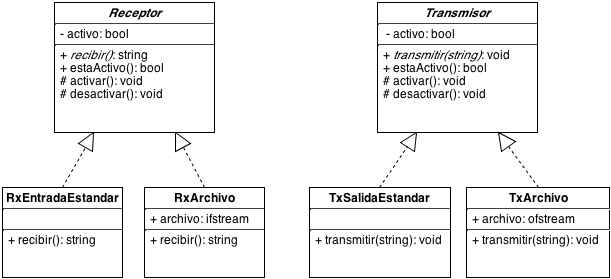
\includegraphics[width=0.75\textwidth]{images/diagrama_2.png}
	\medskip
	\caption{Diagrama de clases de los receptores y transmisores.}
\end{figure}
\bigskip\bigskip\bigskip


	Siguiendo adelante con el modelado de entidades, nos encontramos ahora con posiblemente la mas significativa del sistema ya que con estas se representan las distintas reglas a aplicar sobre las palabras. La clase madre, \textit{Regla} es una clase abstracta de quien heredan todas las demás clases que representan una regla. Todas deben implementar el método virtual \textit{aplicar} de manera de que poliformicamente se apliquen las reglas a cada palabra. Notará el lector que dicho método no recibe un string sino que, en su lugar, recibe una pila de strings. Este peculiar detalle se explica más adelante en la \textit{Sección 3.2}. En la \textit{Figura 2} se muestra un diagrama de clases dicha jerarquía.
\bigskip


% Figura 2
\begin{figure}[h]
	\centering
	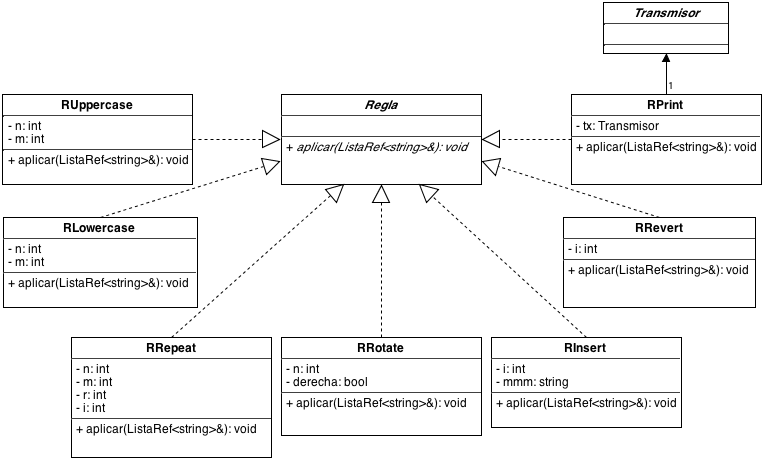
\includegraphics[width=0.87\textwidth]{images/diagrama_3.png}
	\medskip
	\caption{Diagrama de clases de las reglas.}
\end{figure}
\bigskip


\subsection{Recepción y transmisión hacia la I/O Estándar}

	Una de las decisiónes de diseño tomadas fue permitir que el programa se comporte mínimamente como un stream. Con esto nos referimos a que, cuando la recepción se realiza a través de la entrada estándar, a medida que se ingresa una palabra, esta se procesa y es transmitida. En el caso de ser a través de la salida estándar la transmisión, los resultados son emitidos uno a uno a medida que se van ingresando palabras.
	\par
	Con esto se evitó tener que cargar primero todas las palabras a procesar, desembocando inevitablemente en la espera de la generación de resultados por parte del usuario.
\bigskip\medskip



\subsection{Principio básico de funcionamiento}

	El funcionamiento del sistema se centra principalmente en la clase \textit{WordMangling}. Esta contiene como atributo una lista de objetos que son \textit{Regla}.
	\par
	Al darle la orden al objeto WordMangling de ejecutarse el proceso de alteración, se le envía un receptor que le proporcionará las palabras. De esta manera, palabra tras palabra es tratada, transformandola según las reglas contenidas en orden de aplicación en la lista de reglas.
	\par
	Cada resultado de una transformación es apilada en una pila auxiliar. Esta pila es creada por el mismo proceso de WordMangling y es pasada a cada regla (a través del método \textit{aplicar}) debido a que estas últimas deben de poder aplicarse sobre cualquiera de las trasnformaciones previamente realizadas.
\bigskip\medskip


% ESQUEMA DEL DISEÑO
\section{Esquema del diseño}

	A continuación, en la \textit{Figura 3}, se ilustra el diagrama de clases principal que representa la relación entre las entidades que participan del sistema.
\bigskip\bigskip


% Figura 3
\begin{figure}[h]
	\centering
	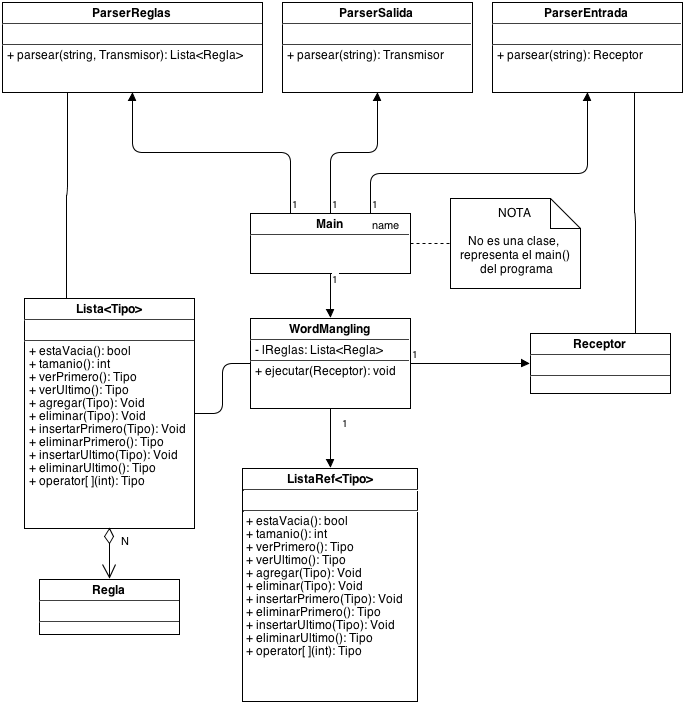
\includegraphics[width=0.87\textwidth]{images/diagrama_1.png}
	\medskip
	\caption{Diagrama de clases general.}
\end{figure}


\end{document}
